%----------------------------------------------------------------------------------------
%	PACKAGES AND OTHER DOCUMENT CONFIGURATIONS
%----------------------------------------------------------------------------------------

\documentclass{article}

\usepackage{fancyhdr} % Required for custom headers
\usepackage{lastpage} % Required to determine the last page for the footer
\usepackage{extramarks} % Required for headers and footers
\usepackage[usenames,dvipsnames]{color} % Required for custom colors
\usepackage{graphicx} % Required to insert images
\usepackage{listings} % Required for insertion of code
\usepackage{courier} % Required for the courier font
\usepackage{lipsum} % Used for inserting dummy 'Lorem ipsum' text into the template
\usepackage{epstopdf}
\usepackage{fancyhdr}
\usepackage{combelow}
\usepackage{enumerate}
\usepackage{amssymb,amsmath}
\usepackage{moreverb}
\usepackage{listings}
\usepackage{multirow}
\usepackage{verbatim}
\usepackage{epsfig}
\usepackage{epstopdf}
\usepackage{tabularx}
\usepackage{color}
\usepackage{subcaption}
\usepackage{tabulary}
\usepackage{wrapfig}
\usepackage{hyperref}
\usepackage[utf8x]{inputenc}

% Margins
\topmargin=-0.45in
\evensidemargin=0in
\oddsidemargin=0in
\textwidth=6.5in
\textheight=9.0in
\headsep=0.25in
\headheight=33pt

\linespread{1} % Line spacing

% Set up the header and footer
\pagestyle{fancyplain}
\fancyhf{}
\lhead{\MNTitle} % Top left header
%\chead{\MNTitleShort} % Top center head
\rhead{
\includegraphics[width=2cm]{Logo.jpg}} % Top right header
\lfoot{\MNClass} % Bottom left footer
\cfoot{} % Bottom center footer
\rfoot{Pagina\ \thepage\ din\ \protect\pageref{LastPage}} % Bottom right footer
\renewcommand\headrulewidth{0.4pt} % Size of the header rule
\renewcommand\footrulewidth{0.4pt} % Size of the footer rule

%----------------------------------------------------------------------------------------
%	CODE INCLUSION CONFIGURATION
%----------------------------------------------------------------------------------------

\definecolor{mygreen}{rgb}{0,0.6,0}
\definecolor{mygray}{rgb}{0.5,0.5,0.5}
\definecolor{mymauve}{rgb}{0.58,0,0.82}

\lstset{ %
  backgroundcolor=\color{white},		% choose the background color; you must add \usepackage{color} or \usepackage{xcolor}
  basicstyle=\small\ttfamily,		% the size of the fonts that are used for the code
  breakatwhitespace=false,			% sets if automatic breaks should only happen at whitespace
  breaklines=true,					% sets automatic line breaking
  captionpos=b,						% sets the caption-position to bottom
  commentstyle=\color{mygreen},		% comment style
  deletekeywords={...},				% if you want to delete keywords from the given language
  escapeinside={\%*}{*)},			% if you want to add LaTeX within your code
  extendedchars=true,				% lets you use non-ASCII characters; for 8-bits encodings only, does not work with UTF-8
  frame=single,						% adds a frame around the code
  keepspaces=true,					% keeps spaces in text, useful for keeping indentation of code (possibly needs columns=flexible)
  keywordstyle=\color{black},			% keyword style
  language=Octave,					% the language of the code
  morekeywords={*,...},				% if you want to add more keywords to the set
  numbers=left,						% where to put the line-numbers; possible values are (none, left, right)
  numbersep=6pt,						% how far the line-numbers are from the code
  numberstyle=\tiny\color{mygray},	% the style that is used for the line-numbers
  rulecolor=\color{black},			% if not set, the frame-color may be changed on line-breaks within not-black text (e.g. comments (green here))
  showspaces=false,					% show spaces everywhere adding particular underscores; it overrides 'showstringspaces'
  showstringspaces=false,			% underline spaces within strings only
  showtabs=false,					% show tabs within strings adding particular underscores
  stepnumber=1,						% the step between two line-numbers. If it's 1, each line will be numbered
  stringstyle=\color{mymauve},		% string literal style
  tabsize=2,							% sets default tabsize to 2 spaces
  title=\lstname						% show the filename of files included with \lstinputlisting; also try caption instead of title
}

% Creates a new command to include a perl script, the first parameter is the filename of the script (without .pl), the second parameter is the caption
\newcommand{\octavescript}[2]{
\begin{itemize}
\item[]\lstinputlisting[caption=#2,label=#1]{#1.m}
\end{itemize}
}

%----------------------------------------------------------------------------------------
%	DOCUMENT STRUCTURE COMMANDS
%	Skip this unless you know what you're doing
%----------------------------------------------------------------------------------------

\setcounter{secnumdepth}{0} % Removes default section numbers
\newcounter{ProblemCounter} % Creates a counter to keep track of the number of problems

\newcommand{\ProblemName}{}
\newenvironment{Problem}[1][Sectiunea \arabic{ProblemCounter}]{ % Makes a new environment called Problem which takes 1 argument (custom name) but the default is "Problem #"
\stepcounter{ProblemCounter} % Increase counter for number of problems
\renewcommand{\ProblemName}{#1} % Assign \ProblemName the name of the problem
\section{\ProblemName} % Make a section in the document with the custom problem count
}{}

\newcommand{\ProblemAnswer}[1]{ % Defines the problem answer command with the content as the only argument
\noindent\framebox[\columnwidth][c]{\begin{minipage}{0.98\columnwidth}#1\end{minipage}} % Makes the box around the problem answer and puts the content inside
}

\newcommand{\SectionName}{}
\newenvironment{Section}[1]{ % New environment for sections within  problems, takes 1 argument - the name of the section
\renewcommand{\SectionName}{#1} % Assign \SectionName to the name of the section from the environment argument
\subsection{\SectionName} % Make a subsection with the custom name of the subsection
}{}

%----------------------------------------------------------------------------------------
%	NAME AND CLASS SECTION
%----------------------------------------------------------------------------------------

\newcommand{\MNTitleShort}{Tema\ \#3} % Assignment title
\newcommand{\MNTitle}{Tema\ \#2 Site web cu chat peste Kubernetes} % Assignment title
\newcommand{\MNDueDate}{Ultimul laborator} % Due date
\newcommand{\MNClass}{SISTEME TOLERANTE LA DEFECTE} % Course/class
\newcommand{\MNClassTime}{} % Class/lecture time
\newcommand{\MNClassInstructor}{Vlad Neculae} % Teacher/lecturer
\newcommand{\MNAuthorName}{Vlad Neculae} % Your name

%----------------------------------------------------------------------------------------
%	TITLE PAGE
%----------------------------------------------------------------------------------------

\title{
%\vspace{2in}
\textmd{\textbf{\MNClass \\ \MNTitle}}\\
\normalsize\vspace{0.1in}\small{Termen de predare: \MNDueDate}\\
}

\date{} % Insert date here if you want it to appear below your name

%----------------------------------------------------------------------------------------

\begin{document}

\maketitle

%----------------------------------------------------------------------------------------
%    TABLE OF CONTENTS
%----------------------------------------------------------------------------------------

%\setcounter{tocdepth}{1} % Uncomment this line if you don't want subsections listed in the ToC

%\newpage
%\tableofcontents
%\newpage


%----------------------------------------------------------------------------------------
%    OBIECTIVELE TEMEI DE CASA
%----------------------------------------------------------------------------------------
\section{Obiective}

Scopul acestei teme este de a implementa, folosindu-vă de Kubernetes si de diferite tehnologii pentru backend, baza de date și frontend, un site web ce conține și un chat.

%----------------------------------------------------------------------------------------
%    PROBLEM 1
%----------------------------------------------------------------------------------------

% To have just one problem per page, simply put a \clearpage after each problem

\begin{Problem}[Enunț]

Această temă este personalizată pentru \textbf{NUMESTUDENT}.

Obiectivul temei este de a crea un website ce conține o aplicație de chat. Tema va fi implementată folosind mai multe deployment-uri peste Kubernetes. Arhitectura acestei aplicații va cuprinde mai multe elemente:

1. Site-ul web efectiv va fi ținut pe un content management system (Wordpress; Joomla; Drupal). Acestei teme îi este asignată \textbf{CMSOPTION} cu \textbf{CMSREPLICAS} replici. Site-ul va fi expus pe portul default (80). Puteți folosi webgui-ul pentru a construi un mic site pentru un magain, o pizzerie, alegerea e a voastra (nu pierdeți mult timp dar nici nu lăsați gol).

2. Sistemul de CMS va folosi o bază de date proprie, pe aceasta o puteți identifica în documentația de pe Docker Hub.

3. Sistemul de chat va fi introdus în pagina web folosind un iframe html. Codul pentru acesta se va afla pe un server web (Php + Apache; Python + Django sau Flask; Node.js).
Acestei teme îi este asignată folosirea \textbf{SERVERWEBOPTION} cu \textbf{SERVERWEBREPLICAS} replici. Chat-ul va fi expus pe portul 88.

4. Mesajele din chat vor fi stocate într-o bază de date (MongDB; MySQL; MariaDB; Postgres; CouchDB; Redis).
Acestei teme îi este asignată folosirea \textbf{DBOPTION}.

\begin{figure}[th]
\centering
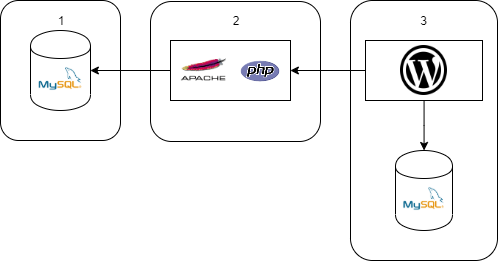
\includegraphics[width=8cm]{architecture_diagram.png}
  \caption{Exemplu de arhitectura pentru aplicatia in discutie}
  \label{fig:architecture_diagram}
\end{figure}

Figura~\ref{fig:architecture_diagram} prezintă o arhitectura în care baza de date aleasă este \textbf{MySql}, backend-ul este alcătuit din \textbf{Php} + \textbf{Apache}, iar layer-ul de prezentare este bazat pe \textbf{Wordpress}, conectat la o baza de date \textbf{MySql}.

\end{Problem}

\begin{Problem}[Detalii implementare]

Pentru majoritatea componentelor este recomandat să folosiți containere de pe Docker hub. În general le puteți folosi cu doar mici modificări. Pentru containerul care ține serverul web ce oferă pagina de chat va trebui să implementați voi codul și să îl adăugați la containerul aferent. Codul va fi implementat în limbajul ales de voi care apare mai sus în acest document.

Tema va consta dintr-un fișier de tip .yaml din care va putea fi pornită prin comanda apply întreaga arhitectură. O dată dat apply totul va trebui să funcționeze. \textbf{Când prezentați nu va fi permis să faceți nici o modificare după ce dați apply, nici măcar la CMS}.

Pentru fiecare componentă se va crea un folder în care se va afla fișierul Dockerfile alături de oricare alte fișiere (cod, export bază de date, șamd).

Recomandare implementare chat:

\begin{enumerate}
    \item Pentru stocarea mesajelor in baza de date, se vor salva următoarele: Mesajul în format text, ASCII; Timestamp-ul trimiterii acestui mesaj.
    \item Pagina de chat va conține un formular în care se introduce un mesaj text, și va avea un buton de send. Mesajele din baza de date vor fi afișate deasupra acestui formular.
    \item Chatul va fi introdus în pagina principală a site-ului printr-un iframe. Pentru a conecta backend-ul cu layer-ul de prezentare, indiferent de tehnologia folosita pentru aceasta ultima componenta, veti folosi un element de tip \textbf{iframe} pentru a afisa pagina primita de la backend.
\end{enumerate}

\end{Problem}


\begin{Problem}[Prezentare și punctare]

În ziua prezentării, mașinile Kubernetes (două) trebuie să fie pregătite și pornite. La fel pentru toate add-on-urile (de ex registry). Containerele ce necesită acest lucru trebuie să fie deja build-uite și puse în registry.

În momentul prezentării va trebui să:
\begin{itemize}
    \item arătați că nu e nici un obiect creat pe cluster;
    \item aplicați .yaml-ul pe cluster;
    \item intrați pe site și arătați că acesta funcționează, că chat-ul merge;
    \item \textbf{NU} aveți voie să faceți nici o configurație la nici una din componente (nici cms).
\end{itemize}

    Distribuția punctajului este următoarea:
\begin{itemize}
    \item 40 puncte - Chat-ul funcționează conform specificațiilor;
    \item 20 puncte - Site-ul integrează tot și funcționează conform specificațiilor;
    \item 30 puncte - Veți primi două-trei instrucțiuni cu operații peste cluster din linia de comandă; Punctajul se primește doar dacă este evident că știți ce faceți și dați comenziile rapid. Va exista un timer. Acest punctaj se dă doar dacă tema funcționează.
\end{itemize}

O arhivă .zip cu toate fișierele va fi pusă la dispoziție pentru verificări plagiat.

\end{Problem}

\end{document}